\documentclass[final]{fhnwreport}       %[mode] = draft or final
                                        %{class} = fhnwreport, article, 
                                        %          report, book, beamer, standalone
%%---Main Packages-----------------------------------------------------------------------
\usepackage[english, ngerman]{babel}	%Mul­tilin­gual sup­port for LaTeX
\usepackage[T1]{fontenc}				%Stan­dard pack­age for se­lect­ing font en­cod­ings
\usepackage[utf8]{inputenc}				%Ac­cept dif­fer­ent in­put en­cod­ings
\usepackage{lmodern}                    %The newer Font-Set
\usepackage{textcomp}					%LaTeX sup­port for the Text Com­pan­ion fonts
\usepackage{caption}					%Customising captions in floating environments
\usepackage{graphicx} 					%En­hanced sup­port for graph­ics
\usepackage{float}						%Im­proved in­ter­face for float­ing ob­jects
\usepackage{ifdraft}                    %Let you check if the doc is in draft mode

%%---Useful Packages---------------------------------------------------------------------
\usepackage{color}						%Colour control for LaTeX documents
\usepackage[pdftex,dvipsnames]{xcolor}  %Driver-in­de­pen­dent color ex­ten­sions for LaTeX
\usepackage{csquotes}                   %Simpler quoting with \enquote{}
\usepackage{siunitx} 					%A com­pre­hen­sive (SI) units pack­age
\usepackage{listings}					%Type­set source code list­ings us­ing LaTeX
\usepackage[bottom]{footmisc}			%A range of foot­note op­tions
\usepackage{footnote}					%Im­prove on LaTeX's foot­note han­dling
\usepackage{verbatim}					%Reim­ple­men­ta­tion of and ex­ten­sions to LaTeX ver­ba­tim
\usepackage[textsize=footnotesize]{todonotes} %Mark­ing things to do in a LaTeX doc­u­ment
\usepackage{titling}					%Control over the typesetting of the \maketitle command

%%---Tikz Packages-----------------------------------------------------------------------
\usepackage{standalone}
\usepackage{tikz}
\usepackage{circuitikz}
\usetikzlibrary{arrows}
\usetikzlibrary{calc}
\usetikzlibrary{intersections}

%%---Math Packages-----------------------------------------------------------------------
\usepackage{amsmath}					%AMS math­e­mat­i­cal fa­cil­i­ties for LaTeX
\usepackage{amssymb}					%Type­set­ting symbols (AMS style)
%\usepackage{amstext}
%\usepackage{amsfonts}
%\usepackage{breqn}
\usepackage{array}						%Ex­tend­ing the ar­ray and tab­u­lar en­vi­ron­ments
\usepackage{amsthm}					%Type­set­ting the­o­rems (AMS style)

%%---Table Packages----------------------------------------------------------------------
\usepackage{tabularx}					%Tab­u­lars with ad­justable-width columns
%\usepackage{longtable}
\usepackage{multirow}					%Create tab­u­lar cells span­ning mul­ti­ple rows
\usepackage{multicol}					%In­ter­mix sin­gle and mul­ti­ple columns

%%---PDF / Figure Packages---------------------------------------------------------------
\usepackage{pdfpages}					%In­clude PDF doc­u­ments in LaTeX
\usepackage{pdflscape}					%Make land­scape pages dis­play as land­scape
\usepackage{subfig}					    %Fig­ures di­vided into sub­fig­ures

%%---Other Packages----------------------------------------------------------------------
%\usepackage{xargs}                     %De­fine com­mands with many op­tional ar­gu­ments


%%---Bibliography------------------------------------------------------------------------
\usepackage[style=ieee,urldate=comp,backend=biber]{biblatex}
\addbibresource{literature/bibliography.bib}

%%---Main Settings-----------------------------------------------------------------------
\graphicspath{{./graphics/}}			%Defines the graphicspath
\geometry{twoside=false}				    %twoside=false disables the "bookstyle"
\setlength{\marginparwidth}{2cm}
\overfullrule=5em						%Creates a black rule if text goes over the margins => debugging




%%---User Definitions--------------------------------------------------------------------
%%Tabel-Definitions: (requires \usepackage{tabularx})
\newcolumntype{L}[1]{>{\raggedright\arraybackslash}p{#1}}    %column-width and alignment
\newcolumntype{C}[1]{>{\centering\arraybackslash}p{#1}}
\newcolumntype{R}[1]{>{\raggedleft\arraybackslash}p{#1}}

%%---Optional Package Settings-----------------------------------------------------------
%Listings-Settings: (requires \usepackage{listings}) => Example with Matlab Code
\lstset{language=Matlab,%
    basicstyle=\footnotesize\ttfamily,
    breaklines=false,%
    morekeywords={switch, case, otherwise},
    keywordstyle=\color{Blue},%
    tabsize=2,
    %morekeywords=[2]{1}, keywordstyle=[2]{\color{black}},
    identifierstyle=\color{Black},%
    stringstyle=\color{Purple},
    commentstyle=\color{Green},%
    showstringspaces=false,%without this there will be a symbol in the places where there is a space
    numbers=left,%
    numberstyle={\tiny \color{black}},% size of the numbers
    numbersep=9pt, % this defines how far the numbers are from the text
    %emph=[1]{word1, word2,...},emphstyle=[1]\color{red}
}							

%Hurenkinder und Schusterjungen verhindern (kein Scherz, Google es)
\clubpenalty10000
\widowpenalty10000
\displaywidowpenalty=10000				                %loads all packages, definitions and settings											
\title{Pflichtenheft}  		        %Project Title
\author{Anklin, Bobst, Horath}      				    %Document Type => Technical Report, ...
\date{\today}          				   %Place and Date

\begin{document}

%%---TITLEPAGE---------------------------------------------------------------------------------
\thispagestyle{empty}
%	\ohead{\includegraphics[scale=0.5]{Bilder/Logo_FHNW.jpg}}
	\begin{figure}
		 \vspace*{-\topskip}\vspace*{-\headsep}
		
\includegraphics[scale=1]{graphics/fhnw_ht_logo_de.pdf}
	\end{figure}
	\begin{center}
		\vspace*{2cm}
		{\huge{\textbf{\thetitle}}}\\
		\vspace*{0.5cm}
		
		{\huge{\textbf{Bluetooth Mesh network for automation applications}}}\\
		\vspace*{0.5cm}
		
		{\scshape\Large Projekt 5 - \theauthor \\} \Large{\today}
		\vfill
		\begin{normalsize}
			{\begin{tabbing}
<<<<<<< HEAD
					\textbf{Auftraggeber:} \hspace{5cm}\= 
					\>Cyrill Horath \\ 
					\>Raffael Anklin \\ 
					\>Robin Bobst \\ 
					\\[0.8cm]
					
					\\[0.8cm]
					\textbf{Projektbetreuer:} 
=======
					\textbf{Auftraggeber:} \hspace{5cm}\= Matthias Meier\\
					
					\\[0.8cm]
					\textbf{Fachcoach:} 
>>>>>>> f69a74c837fcb7c8bd9cb53dd040188b1bebb85d
					\>Matthias Meier\\
					\>Manuel Di Cerbo\\
					
					\\[0.4cm]
<<<<<<< HEAD
					\textbf{Projektleiter:} \>???\\
					\\[0.4cm]
					
					\textbf{Team:} 
					\>Cyrill Horath \\ 
					\>Raffael Anklin \\ 
					\>Robin Bobst \\ 
=======

					
					\textbf{Team:} \>Raffael Anklin \\ \>Robin Bobst \\ \>Cyrill Horath \\ 
>>>>>>> f69a74c837fcb7c8bd9cb53dd040188b1bebb85d
					\\[0.8cm]
					
					\textbf{Studiengang:} \>Elektro- und Informationstechnik
					\\[0.8cm]	\textbf{Semester:} \>Herbstsemester 2019
			\end{tabbing}}
		\end{normalsize}
		\vfill
	\end{center}
\clearpage


%%---TABLE OF CONTENTS-------------------------------------------------------------------
\pagenumbering{Roman}		
\selectlanguage{ngerman}				%ngerman or english
\tableofcontents
\clearpage

%%---TEXT--------------------------------------------------------------------------------
\pagenumbering{arabic}
	\clearpage
\section{Übersicht}\label{sec:Uebersicht}

In diesem Kapitel soll eine Übersicht über den Inhalt des Projekt 4 des Studiengangs Elektro- und Informationstechnik gegeben werden. Dabei soll auch aufgezeigt werden, welche Ziele erreicht werden sollen und welche Lieferobjekte erstellt werden müssen. 

 









	
\subsection{Ausgangslage}\label{subsec:Ausgangslage}

Die Bluetooth Technik wurde im Jahr 1998 von der "Bluetooth Special Interest Group" (SIG) als Industriestandart für Datenübertragung herausgebracht. Ursprünglich wurde das Funkverfahren jedoch von Jaap Hartsen und Sven Mattisson für die Firma Ericsson entwickelt. Der Hauptzweck dieser Methode zur Datenübermittlung war das Ersetzen von Kabelverbindungen von Mobiltelefone, Peripheriegeräte oder Computer. Der Name Bluetooth oder auf Deutsch Blauzahn kommt vom dänischen König Harald Blauzahn. Diesem König gelang es die verfeindeten Länder Dänemark und Norwegen dank seiner Kommunikationsfreudigkeit zu vereinen. Da die skandinavischen Firmen Nokia und Ericsson viel Aufwand in die Bluetooth Technologie gesteckt haben, wurde dieser Name sowie die Runen H (Harald) und B (Blauzahn) für das Logo übernommen.\cite{michna_entwicklungsgeschichte_2019} Seit dem Start von Bluetooth gab es eine Vielzahl von Versionen, die von mehreren Firmen ständig weiterentwickelt werden. Im Dezember 2009 wurde von der SIG die Version 4.0 Smart vorgestellt. Mit dieser Version von Bluetooth war es möglich kleine und sparsame Geräte wie z.B. smarte Uhren, Brillen oder sogar Ringe herzustellen.\cite{bluetooth_sig_our_2019} Ab dem Update Bluetooth 5.0 im Jahre 2016, ist es möglich Bluetooth Komponenten in einem Mesh-Netzwerk zu konfigurieren. Dieses Netzwerk basiert auf einem "many-to-many pairing system" d.h. jeder Teilnehmer ist mit den anderen Teilnehmern verbunden. Dieses dezentralisierte System hat den Vorteil, dass es kein Master Element benötigt. Fällt ein Teilnehmer aus besteht das Netzwerk trotzdem weiter.\cite{woolley_intro_2017} Genau hier soll das Projekt 5 ansetzten. Da die Programmierung eines Mesh-Netzwerkes sehr kompliziert ist, wird dafür eine "'Open Source Software"' geschrieben, die es ermöglicht ein Netzwerk vereinfacht aufzubauen und zu konfigurieren.

\todo [inline]{Überarbeitung Einführung Mesh-Standard. Gibt es Mesh erst ab BT 5 oder schon mit BT 4? Oder ist es nur abhängig ob BLE vorhanden ist?}








	\clearpage
\subsection{Projektziele}\label{subsec:Projektziele}
In den beiden Tabellen \ref{tab:Pflichtziele} und \ref{tab:Wunschziele} sind die Pflicht- resp. Wunschziele für dieses Projekt festgehalten.

\begin{table}[H]
\begin{tabular}{ | C{0.9cm} | p{3.3cm} | p{10cm} |}
	\hline
	\multicolumn{3}{|l|}{\textbf{Pflichtziele}}\\ \hline
\textbf{Nr.}& \textbf{Ziel}& \textbf{Beschrieb}\\ \hline

P1 & Bluetooth-Mesh-Netzwerk & Eine variable Anzahl an BLE-Nodes bauen ein Mesh-Netzwerk auf um darin Datenaustausch zu ermöglichen.\\ \hline

P2 & UPN & Der Universal-Peripheral-Node kann je nach Einsatz als Sensor oder Aktor konfiguriert und bestückt werden.\\ \hline

P3 & Low Power & Die UPN sind bezüglich Hardware und Software energiesparend konzipiert um sie autonom betreiben zu können.\\ \hline

P4 & Security & Das Mesh-Netzwerk ist gegen unerlaubten Zugriff und sonstigen Angriffen geschützt.\\ \hline

P5 & Netzunabhängig & Durch Versorgung mittels Batterie und Energy-Harvesting können die UPN komplett netzunabhängig betrieben werden.\\ \hline

P6 & Energy-Harvesting & Für die Versorgung der UPN werden verschiedene Varianten für das Energy-Harvesting entwickelt. Das Ergebnis wird eine Variantenstudie sein.\\ \hline

P7 & Gateway & Zur Konfiguration des Bluetooth-Mesh-Netzwerks steht ein Gateway basierend auf Standard Hardware (Raspberry-Pi + nRF52840 USB Dongle o.ä.) zur Verfügung.\\ \hline
    
P8 & LAN/WLAN & Für die Integration in TCP/IP basierte Systeme bietet der Gateway eine entsprechende Schnittstelle.\\ \hline

P9 & CLI & Mittels Command-Line-Interface kann das Mesh-Netzwerk verwaltet werden.\\ \hline

\end{tabular}\\
\caption{Pflichtziele}
\label{tab:Pflichtziele}
\end{table}


\begin{table}[H]
\begin{tabular}{ | C{0.9cm} | p{3.3cm} | p{10cm} |}
	\hline
	\multicolumn{3}{|l|}{\textbf{Wunschziele}}\\ \hline
\textbf{Nr.}& \textbf{Ziel}& \textbf{Beschrieb}\\ \hline
    	 
    
W1 & UPN Konfiguration via Mesh & Einstellungen des UPN können via Mesh Netzwerk angepasst werden und somit z.B. die Peripheriekonfiguration verändert werden.\\ \hline

W2 & Firmwareupgrade via Mesh & Die Firmware der UPN wird via Mesh-Netzwerk aktualisiert. \\ \hline

W3 & BLR und BLE & Bluetooth Long Range (BLR) und Bluetooth Low Energy (BLE) ergänzen das Bluetooth Mesh um die Reichweite zu vergrössern oder den Energieverbrauch nochmals zu vermindern. \\ \hline

W4 & Dedizierte Hardware UPN & Das UPN ist als dedizierte Hardware realisiert und somit einsatzbereit. \\ \hline

W5 & Datenschnittstelle & Mittels passender Datenschnittstelle auf dem Gateway können Fremdsysteme wie Apple Homekit, Google Home oder KNX angebunden werden.\\ \hline

W6 & UDP Kommunikation & Damit keine Daten auf dem Gateway zwischen gespeichert werden müssen können die Nodes mittels beliebigem UDP Protokoll (MQTT, CoAP, usw.)direkt mit Fremdsystemen kommunizieren.\\ \hline

W7 & HMI & Ein Human-Machine-Interface in Form einer Webapplikation unterstützt den User bei der Konfiguration des Mesh-Netzwerks und ermöglicht die Anbindung an Fremdsysteme. \\ \hline

W8 & Dedizierte Gateway Hardware & Der Gateway ist auf einer dedizierten Hardware umgesetzt. \\ \hline

W9 & Onboard Bluetooth & Da der Raspberry-Pi 4 bereits ein Bluetooh 5 Chip besitzt soll direkt dieser verwendet werden anstelle eines angeschlossenen Dongles. \\ \hline

W10 & Mobiltelefon & Anstelle oder ergänzend zum Gateways kann ein Mobiltelefon ins Mesh-Netzwerk eingebunden werden um Konfigurationen vorzunehmen oder Daten aus zu lesen. \\ \hline

W11 & GSM/LTE & Für Feldanwendungen besitzt der Gateway ein GSM/LTE Modul. \\ \hline

W12 & Versuchsaufbau Energy-Harvesting & Erfolg versprechende Energy-Harvesting-Systeme werden in einem Versuchsaufbau auf deren Tauglichkeit weiter geprüft. \\ \hline


\end{tabular}\\
\caption{Wunschziele}
\label{tab:Wunschziele}
\end{table}


\todo [inline]{Bitte Ziele durchlesen und allenfalls Anpassungen vornehmen. RA OK!}
















	\clearpage
\subsection{Lieferobjekte}\label{subsec:Lieferobjekte}
Zusätzlich zu den Projektzielen, folgen in diesem Kapitel die Lieferobjekte und wichtige Meilensteine mit dem jeweiligen Datum. In der Tabelle \ref{tbl:Lieferobjekte} sind diese detailliert aufgelistet.  


\begin{table}[H]
     \centering
\begin{tabular}{|c|c|l|}\hline
   \textbf{Nr.} & \textbf{Datum} & \textbf{Lieferobjekt} \\ \hline
   1 & 17.03.2019 & Abgabe Fachliches Pflichtenheft, erste Version \\ \hline 
   2 & 31.03.2019 & Abgabe Fachliches Pflichtenheft, definitive Version \\ \hline
   3 & 05.05.2019 & Abgabe Disposition und Einleitung Fachbericht \\ \hline
   4 & 07.05.2019 & G-Code drahtlos übermitteln \\ \hline   
   5 & 19.05.2019 & Abschluss Realisierung \\ \hline   
   6 & 02.06.2019 & Abschluss Validierung \\ \hline   
   7 & 11.06.2019 & Abgabe Fachbericht \\ \hline
   8 & 11.06.2019 & Abgabe Fact sheet \\ \hline
   9 & 11.06.2019 & Abgabe Produkt und dazugehörige Software \\ \hline   
   
 \end{tabular}
     \caption{Lieferobjekte und wichtige Meilensteine}
     \label{tbl:Lieferobjekte}
\end{table}

\todo[]{asdlöf}








\pagebreak

\clearpage
\section{Lösungskonzept}\label{sec:Loesungskonzept}
In Abbildung \ref{img:Grobkonzept} ist das Blockschaltbild ersichtlich, welches alle Teilsysteme und Einheiten darstellt. Es ist modular gegliedert und bietet eine Übersicht der Schnittstellen zwischen den einzelnen Modulen. 

Das Lösungskonzept besteht aus physikalisch getrennten \textit{"Nodes"} (Knöten), dem \textit{Gateway Interface System} (GIS) und dem \textit{Universal Peripherial Node} (UPN). , das \textit{Human Maschine System} (HMS) und den Drucker selbst, einen \textit{Ender 3} der Firma \textit{Creality3D}. 

Der UPN bildet den Hauptbestandteil des Lösungskonzepts. Es beinhaltet die Druckersteuerung und die Kommunikationsschnittstellen. Um diese zwei Aufgaben zu separieren befinden sich zwei Mikroprozessoren in dieser Einheit. Zusätzlich werden die Aktoren und Sensoren des 3D-Druckers  angesteuert und eingelesen. Eine Statusanzeige zur Visualisierung des Zustandes ist ebenfalls angedacht.

Das HMS bildet die Benutzerschnittstelle über ein internetfähiges Gerät. Es kommuniziert mittels WLAN mit dem MCS. Über dieses Gerät können Druckaufträge verwaltet und überwacht werden. Auf dem 3D-Drucker befinden sich alle Aktoren und Sensoren. Sie werden über Kabelverbindungen an das MCS angebunden.



\begin{figure}
	\centering
	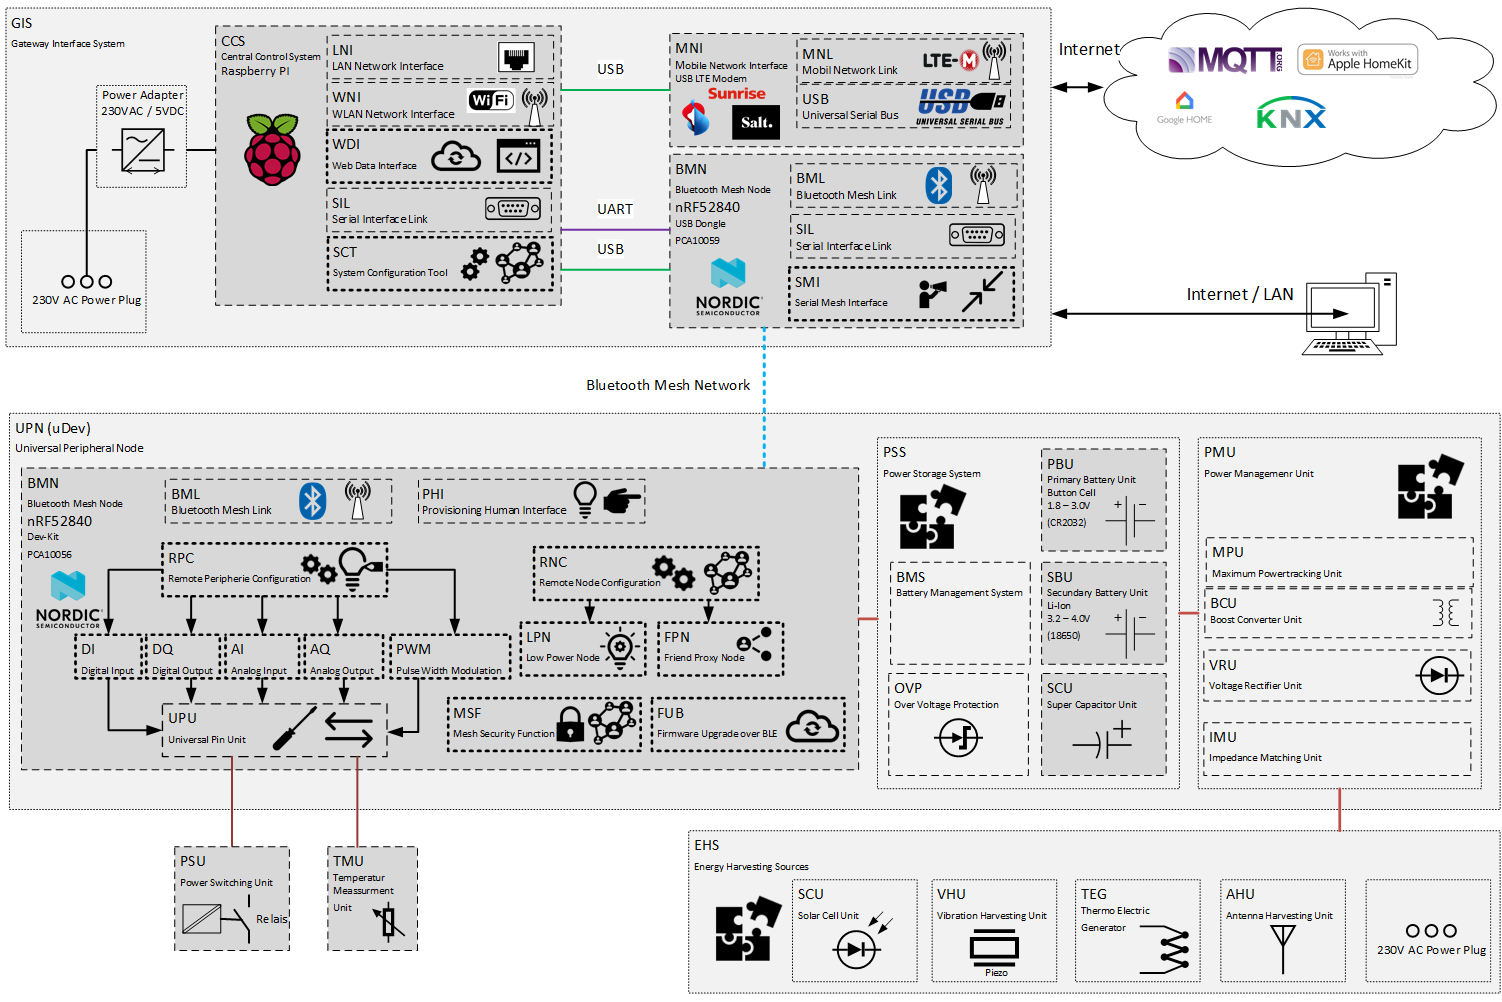
\includegraphics[scale=0.60,angle=90]{19HS-pro5E-TeamBlau_Grobkonzept_02102019_Backup_ohne_Rahmen.png}
	\caption{Blockschaltbild des Lösungskonzepts}
	\label{img:Grobkonzept}
\end{figure} 









\pagebreak

\clearpage
\section{Hardware}\label{sec:Hardware}
In diesem Kapitel wird die Hardware vom \textit{Gateway Interface System}, dem \textit{Universal Peripheral Node}, dem \textit{Energy Harvesting System} und dem \textit{Power Storage System} beschrieben. 


\subsection{Bluetooth Mesh Node (BMN)}\label{subsec:BMN}
Im Bluetooth Mesh Protokoll gibt es zwei verschiedene  Geräte, ein \textit{"'unprovisioned device"'} und einen \textit{"'Node"'}. Das \textit{"'unprovisioned device"'}  ist ein Teilnehmer, der unbekannt für das Mesh Netzwerk ist und deshalb keine Rechte besitzt. Wird dieses Gerät nun in das Netzwerk aufgenommen, so wird das \textit{"'unprovisioned device"'}  zu einem \textit{"'Node"'}. Dieses vorgehen nennt sich \textit{"'provisioning"'}.\cite{afaneh_ultimate_2018} Die Hardware für den \textit{"'Node"'} besteht bei allen Geräten aus dem gleichen SoC. Der nRF52840 von Nordic Semiconductor eignet sich aus folgenden Gründen perfekt für diese Anwendung. Die \textit{"'Nodes"'}. dürfen um eine lange Laufzeit zu generieren, sehr wenig elektrische Leistung beziehen. Der NRF52840 benötigt im Ruhemodus nur wenige $[\mu A]$. Ein weiterer Grund ist die sehr gute Dokumentation der Software von Nordic Semiconductor. Die gesamte Software ist im Infocenter erhältlich und frei zugänglich. Weitere Vorteile befinden sich in der Tabelle \ref{tbl:Vorteilte_nRF52}:\cite{nordic_semiconductor_nrf52840_2019} \\

\cite{jaeger_was_2018}

\begin{table}[h]
	\begin{tabular}{ll}
		\multicolumn{2}{l}{{\ul \textbf{Vorteile des nRF52840}}}       \\
		Bluetooth 5                          											   & -95 dBm Sensivität      \\
		Multiprotokoll (Thread, Zigbee, usw) 						   & +8 dBm Ausgangsleistung \\
		Geringer Stromverbrauch  (wenige $[\mu A]$)      	& USB 2.0                 \\
		12bit ADC                            												& NFC                     \\
		1 MB flash und 256kB RAM Speicher    						& ARM M4F Cortex         
	\end{tabular}
	\caption{Vorteile des nRF52840}
	\label{tbl:Vorteilte_nRF52}
\end{table}


\begin{figure}[h]
	\centering
	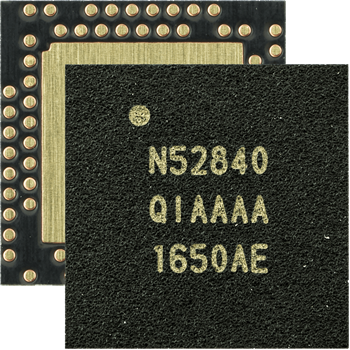
\includegraphics[scale=0.5,angle=0]{nRF52840.png}
	\caption{nRF52840 SoC}
	\label{img:nRF52840}
\end{figure} 


\subsection{Energy Harvesting System (EHS)}\label{subsec:EHS}

Das \textit{EHS} beinhaltet fünf unterschiedlichen Methoden um Energie aus der Umgebung aufzufangen. Diese sind in der folgenden Tabelle mit den wichtigsten Kenndaten aufgefasst. 

\begin{table}[H]
	\centering
	\begin{tabular}{|c|c|l|l|l|}\hline
		\textbf{Quelle} & \textbf{Leistungsdichte} & \textbf{Technologie} & \textbf{Vorteile} & \textbf{Nachteile} \\ \hline
		
		Solar & Innenbereich: 10  $\mu$W/cm2  \newline Aussenbereich: 10 mW/cm2 & Photovoltaic & Hohe Leistungsdichte \newline Ausgereift & Nicht immer verfügbar \newline Benötigt exponierte Oberfläche (nicht Implementierbar) \newline Teuer \\ \hline
		
		Vibration & Mensch: 4 $\mu$W/cm2 \newline Industrie: 100 $\mu$W/cm2 & Piezoelektrisch \newline Elektrostatisch \newline Elektromagnetisch & Implementierbar \newline Hohe Effizienz & Nicht immer verfügbar \\ \hline
		
		
		
	\end{tabular}
	\caption{Lieferobjekte und wichtige Meilensteine}
	\label{tbl:Lieferobjekte}
\end{table} 
\pagebreak

\clearpage
\section{Software}\label{sec:Software}
Das Kapitel Software befasst sich mit der Programmierung des Mikrocontroller \textit{NRF52840} sowie des Gateway Interface System.

\subsection{Software Development Kit for NRF52}\label{subsec:SDK}
Text Robin

\subsection{Human Machine System (HMS)}\label{subsec:HMS_SW}
\pagebreak

\clearpage
\section{Bedienung}\label{sec:Bedienung}
Der 3D-Drucker kann entweder durch das webbasierte GUI oder über ein eingebautes Display mit einem Drehgeber gesteuert werden, welche auf der Leiterplatte verbaut sind. Die jeweils verfügbaren Funktionen und Einstellungen sind identisch. Weiterhin können G-Code Dateien wahlweise mittels WLAN oder einer SD-Karte übergeben werden. 

Die Standardansicht des Displays und des GUIs bildet die Statusanzeige. Auf ihr werden aktuelle Daten wie Temperatur des Extruders und des Heizbetts, Ventilatorgeschwindigkeit, Multiplikator Geschwindigkeit, Multiplikator Zufuhr und Druckfortschritt angezeigt. Durch Druck auf den Drehgeber wird eine Liste von verschiedenen Menüs geöffnet. Diese werden als \textit{Kurzeinstellungen}, \textit{SD-Karte} und \textit{Position} bezeichnet. In \textit{Kurzeinstellungen} sind häufig verwendete Einstellungen und Funktionen zu finden, wie etwa \textit{Vorheizen ABS/PLA}, \textit{Abkühlen}, \textit{Deaktiviere Schrittmotoren}, \textit{Home All} oder \textit{Druckauftrag Abbrechen}. 

Im Menü \textit{SD-Karte} stehen die Funktionen  \textit{Mount/Unmount SD-Karte}, \textit{Drucke Datei}, \textit{Lösche Datei}. zur Verfügung. Das Menü \textit{Position} bietet verschiedene Funktionen wie etwa \textit{Bewege x,y,z}, \textit{Home x,y,z} und \textit{Home alle}, mit welchen die Achsen unabhängig voneinander bewegt und ihre Ausgangslage zurückversetzt werden können.
\pagebreak











\pagebreak

\clearpage
\section{Projektvereinbarung}\label{sec:Projektvereinbarung}
	\begin{tabbing}
		\textbf{Projektcoach}\\[0.2cm]
		Meier Matthias\\[0.2cm]
		Ort, Datum: \hspace{5cm}\=Unterschrift:
		\\[0.5cm]----------------------------- \>-----------------------------
		\\[0.2cm]
		Di Cerbo Manuel\\[0.2cm]
		Ort, Datum: \hspace{5cm}\=Unterschrift:
		\\[0.5cm]----------------------------- \>-----------------------------
		\\[1cm]
		\textbf{Projektteam}\\[0.2cm]
		Anklin Raffael\\[0.2cm]
		Ort, Datum: \>Unterschrift:
		\\[0.5cm]----------------------------- \>-----------------------------
		\\[0.2cm]
		Bobst Robin\\[0.2cm]
		Ort, Datum: \>Unterschrift:
		\\[0.5cm]----------------------------- \>-----------------------------
		\\[0.2cm]
		Horath Cyrill\\[0.2cm]
		Ort, Datum: \>Unterschrift:
		\\[0.5cm]----------------------------- \>-----------------------------
	\end{tabbing}
	
	\clearpage






\clearpage
%%---BIBLIOGRAPHY------------------------------------------------------------------------
{\sloppypar
\printbibliography
\label{sec:lit}
%\selectlanguage{ngerman}				%ngerman or english
%\printbibliography
}

%%---APPENDIX----------------------------------------------------------------------------
\begin{appendix} 


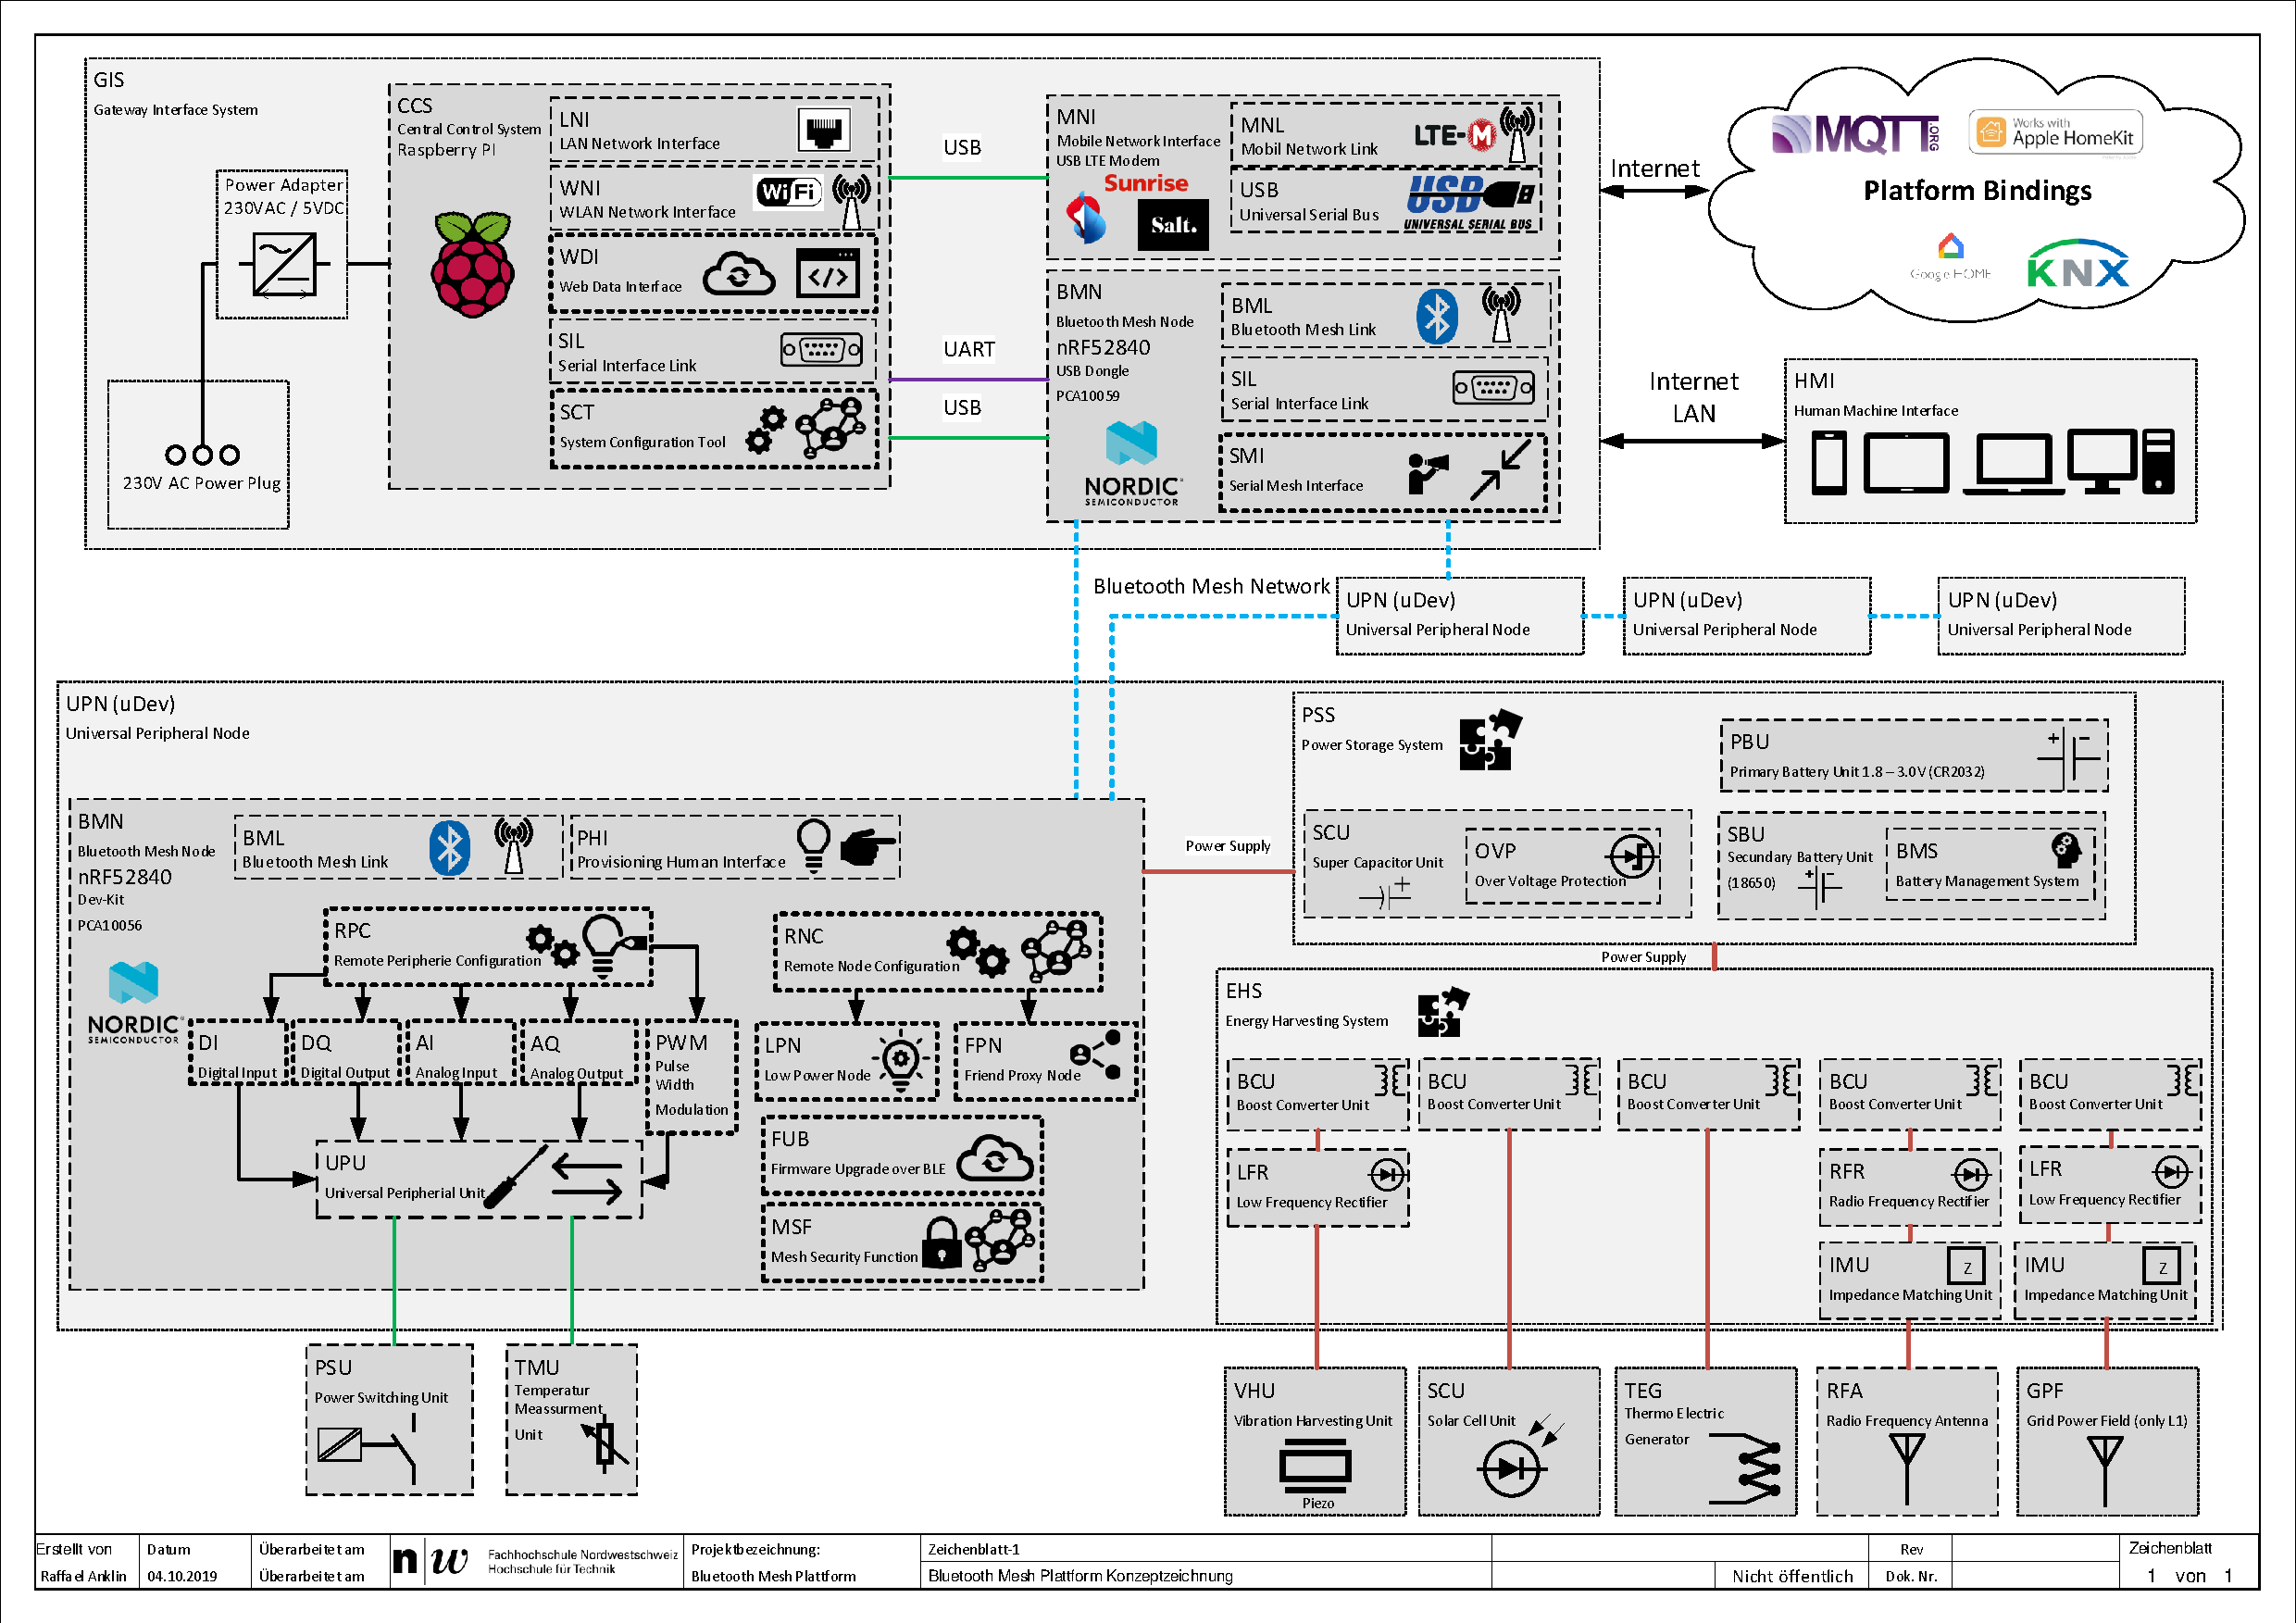
\includepdf[pages={1}, nup=1x1, landscape=true, scale=0.8 ,offset=6 -30, pagecommand={\section{Konzeptschema}\label{app:Konzeptschema}\thispagestyle{myheadings}}]{19HS-pro5E-TeamBlau_Grobkonzept_04102019.pdf}


\end{appendix}


%%---NOTES for DEBUG---------------------------------------------------------------------
\ifdraft{%Do this only if mode=draft
%%requires \usepackage{todonotes})
\newpage
\listoftodos[\section{Todo-Notes}]
\clearpage
}
{%Do this only if mode=final
}

\end{document}
